\section{Introduction}
%\begin{figure}
%    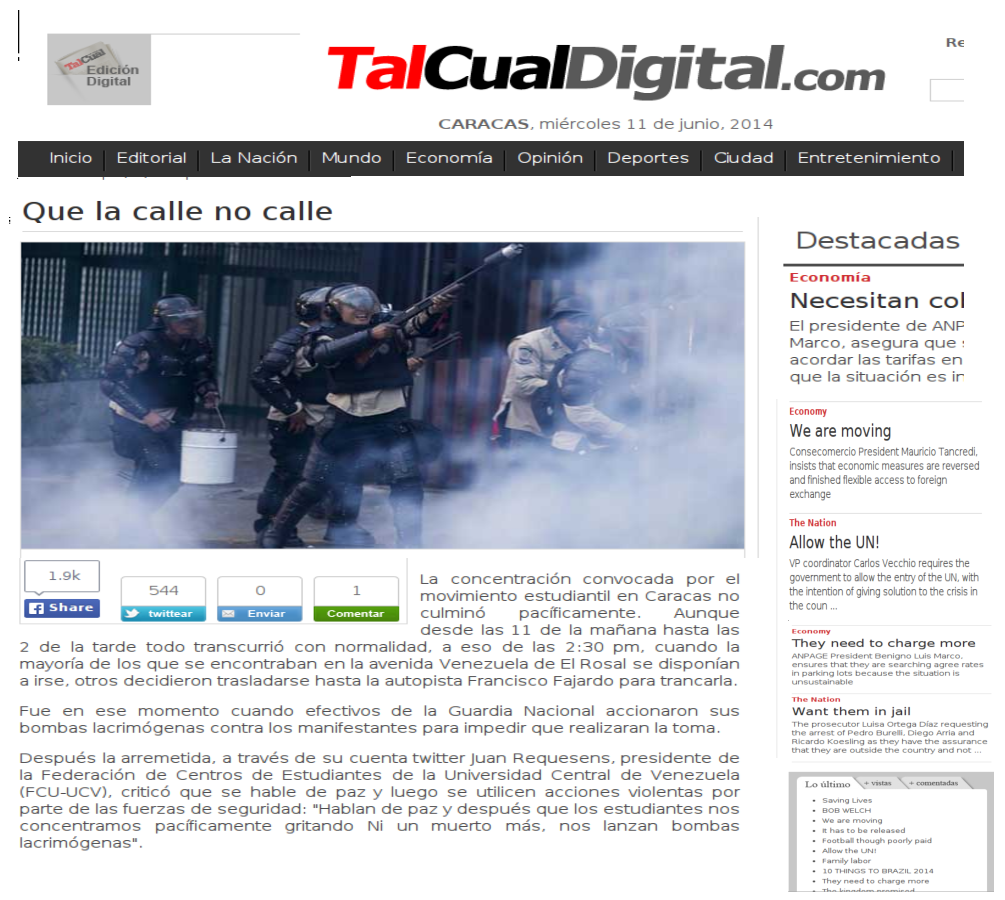
\includegraphics[width=0.5\textwidth, height=0.4\textwidth]{pp_example}
%    \caption{An example article describing plans for a future protest (Venezuela, June 11, 2014).}
%    \vspace{-2em}
%    \label{pp_example}
%\end{figure}
Civil unrest (protests, strikes, and ``occupy'' events) is a common happening in both democracies
and authoritarian regimes.
Although we typically associate civil unrest with disruptions and instability, for a social scientist
civil unrest reflects the democratic process by 
which citizenry communicate their views and preferences to those in authority. 
The advent of social
media has afforded citizenry new mechanisms for organization and mobilization, and online news sources
and social networking sites like Facebook and Twitter
can provide a window into civil unrest happenings in a particular country.

\subsubsection{Why study and forecast protests?}
Our region of interest is Latin America and protest
is an important topic of study here,
as many countries here are democracies struggling to consolidate themselves. The combination of weak channels of communication 
between citizen and government, and a citizenry that still has not grasped the desirability of elections as the means to affect politics 
means that public protest will be an especially attractive option. To 
illustrate the power of protest in Latin America we need only recall 
that between 1985 and 2011, 17 presidents resigned or were impeached under pressure from demonstrations, usually violent, in the streets. Protests have 
also resulted in the rollback of price increases for public services, such as during the ‘Brazilian Spring’ of June 2013.

Forecasting protests is an important capability in many domains.
For the tourism industry, forecasting protests can
support the issuance of travel warnings. For law enforcement,
forecasting protests can aid in preparedness. For the social scientist,
protests forecasts will provide insight into how citizens express themselves.
For the government, a protest forecasting system can help prioritize
citizen grievances. Finally, protests can have a debilitating effect on
multiple industries (esp. those that rely on worldwide supply chain management)
and thus a protest forecasting system can aid in planning and design
of alternative travel and shipping routes.

\subsubsection{Planned protests}
Our basic hypothesis is that
protests that are larger will be more disruptive and communicate support for its cause better than smaller protests. 
Mobilizing large numbers of people is more likely to occur if a protest is organized and the time and place announced in
advance. Because protest is costly and more likely to succeed if it is large, we should expect planned, rather than 
spontaneous, protests to be the norm. Indeed, in a sample of 288 events from our study selected for qualitative review of their antecedents,
for 225 we located communications regarding the upcoming occurrence of the event in media, and only 49 could be classified as 
spontaneous (we could not determine whether communications had or had not occurred in the remaining 14 cases).

\subsubsection{EMBERS}
We are an industry-university partnership charged with developing an
automatic protest forecasting system for 10 countries in
Latin America. Our system, called EMBERS, has been
deployed since Nov 2012 and has been generating forecasts (called
warnings or alerts) automatically, without a human-in-the-loop. These forecasts are emailed to
a third party (MITRE) for evaluation. Analysts at MITRE organize a reference
database of protests (called the Gold Standard Report,
or GSR) by surveying newspapers for reportings of protests, and
compare our warnings against the GSR to generate a scoring report (evaluation
criteria described later).

The full EMBERS system has been described elsewhere~\cite{emberskdd}, including
the overall system architecture, data sources used for analysis, and the
various forecasting models in EMBERS. EMBERS adopts a multi-model approach,
wherein different models are leveraged for their selective superiorities
to generate a fused set of alerts. Arguably, one of the
best performing models in EMBERS is the planned protest model that detects
ongoing organizational activity and generates warnings accordingly. This paper
is the first to present this model in detail, including the 
research issues involved, and how we addressed them in EMBERS.

Capturing mentions of protest planning and organization 
is not as easy as it might appear. First, articles of interest are written in
different languages (Spanish, Portugese, French, Dutch, and English). 
Second, multiple locations are often mentioned in a given article, leading
to (natural language) ambiguity about the intended location of the event.
Significant reasoning is required to discern the correct protest location.
Finally, dates are often described in relative terms, e.g., `Sunday' and 
thus these vague references need to be resolved into absolute temporal
information. 

Our detection approach 
combines shallow linguistic analysis to identify a corpus of relevant
documents (articles, tweets) which are then subject to targeted deep semantic analysis.
Despite its simplicity, we are able to
detect indicators of event planning with surprisingly high
accuracy. Our contributions are:

\iffalse
\begin{figure}
    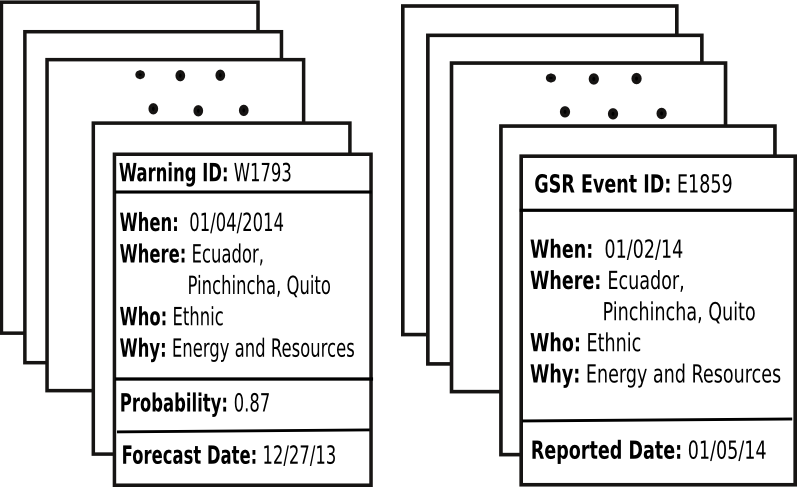
\includegraphics[width=0.5\textwidth]{alertstructure}
    \vspace{-2em}
    \caption{An example warning (left) and GSR event (right).}
    \label{fig:alertstructure}
\end{figure}
\fi

\begin{enumerate}
\item We present a protest forecasting system that couples three key technical ideas:
key phrase learning to identify what to look for, probabilistic soft logic to reason about location occurrences in extracted results, and 
date normalization to resolve future tense mentions. We demonstrate how the integration of these ideas achieves objectives in precision,
recall, and quality (accuracy).
\item We illustrate the application of our system to 10 countries in Latin America, viz. Argentina, Brazil, Chile, Colombia, Ecuador, El Salvador, Mexico, Paraguay, Uruguay, and Venezuela. Our system predicts the {\it when} of the protest
as well as {\it where} of the protest (down to a city level granularity).
%See Fig.~\ref{fig:alertstructure} for an example.
We conduct ablation studies to identify the 
relative contributions of news media (news + blogs) versus social media (Twitter, Facebook) to identify future happenings of
civil unrest. Through these studies we illustrate the selective superiorities of different sources for specific countries.
\item Unlike many studies of retrospective forecasting of protests,
our system has been {\bf deployed and in operation for nearly two years.}
The end consumers of our alerts are analysts studying Latin America.
%To assess the forecasting prowess of our approach,
%we calculate the lead time from when the forecast is made to
%the actual event date, 
Our results demonstrate that we are able to 
capture significant societal unrest in the above countries with an average lead time of 4.08 days. 

\end{enumerate}

